\documentclass[a4paper]{report}

\usepackage[nottoc,numbib]{tocbibind}
\usepackage{graphicx}

\begin{document}

\title{Automatic Structural Inference of Network Protocols}
\author{Fredrik Appelros \and Carl Ekerot}
\date{\today}
\maketitle

\begin{abstract}
An abstract is a brief summary of a research article, thesis, review,
conference proceeding or any in-depth analysis of a particular subject or
discipline, and is often used to help the reader quickly ascertain the paper's
purpose.
\end{abstract}

\tableofcontents

\chapter{Introduction}

\section{Background}
Here we will write a formal introduction to network protocols and why network
protocol inference is needed. Also explain what protocol inference is, of
course.

\section{Related work}
Here is a discussion about related work. We talk about different methodologies
along with their respective advantages and disadvantages. As an example here
is a citation \cite{cui07}.

\chapter{Method}

\section{Approach}
Here we will write how we approched the problem of network protocol inference
and the different components that comprise our method. Start with explaining
why we need to cluster our data and continue to explain what needs to be done
after the clustering step to actually achieve protocol inference.

\section{Clustering}

\subsection{Cluster theory}
Here we will explain in general terms what clustering is and what it is used
for.

\subsubsection{K-means}
The K-means algorithm is explained here as an example of a simple clustering
algorithm. The section is concluded with a practical example.

\subsection{Features}
The term feature is explained here and one can draw parallels to how we use
raw data in the K-means example above where that is the most basic kind of
feature.

\subsubsection{High dimensional data}
Continue to build upon the simple idea of two dimensional clustering and
introduce new problems where the number of dimensions are significantly
higher.

\subsubsection{Principal component analysis}
Introduce principal component analysis (PCA) and explain how it can relieve
some of the issues that occurs in high dimensional clustering. End with an
example of how this can be done in practice with our choice of features on a
set of data taken from DNS traffic.

\subsection{Hierarchical clustering}
Introduce the concept of hierarchical clustering and how different clusters
may be related to one another.

\subsubsection{Unweighted Pair Group Method with Arithmetic Mean}
Use the Unweighted Pair Group Method with Arithmetic Mean (UPGMA) as an example
of hierarchical clustering. Show how it fares well on our DNS data used in the
PCA section but note clearly the problem with extracting clusters from the tree
structure.

\subsection{Density-based clustering}
Explain the basic idea of density-based clustering.

\subsubsection{DBSCAN}
Continue to describe the DBSCAN algorithm as a practical implementation of the
ideas introduced in the section above. Conclude with an example based on the
same DNS data as before. Be sure to mention the problem with using the method
on unknown data as the parameters needs to be fine tuned.

\subsubsection{OPTICS}
Introduce the OPTICS algorithm which is an extension to the DBSCAN algorithm
that marries the concepts of hierarchical clustering with density-based
clustering. Emphasize the advantage of more robust parameters but also the
disadvantage of yet again introducing the problem of cluster extraction.

\paragraph{Cluster extraction}
Explain that the problem with cluster extraction can be solved in OPTICS in
contrast to UPGMA. Start with the most basic threshold extraction and continue
with the more advanced hierarchical extraction method. Conclude with an example
of cluster extraction from DNS data.

\section{Field analysis}

\subsection{Byte distribution}
Explain how we reached the decision to use byte distributions in our attempts
to find structures in protocols.

\subsection{Field classes}
Introduce the classes of fields that we have established as identifiable. Use
plots of their byte distributions to motivate our decision.

\subsection{Linear models}
Explain what a linear model is and how we use it to model the relationship
between length fields and message lengths.

\subsubsection{Linear regression}
Explain how one can fit a linear model to data using regression. Mention the
problem with noise.

\subsubsection{RANSAC}
Explain how the RANSAC algorithm works and how it can be used to solve the
problem with fitting a linear model in noisy data.

\begin{figure}
    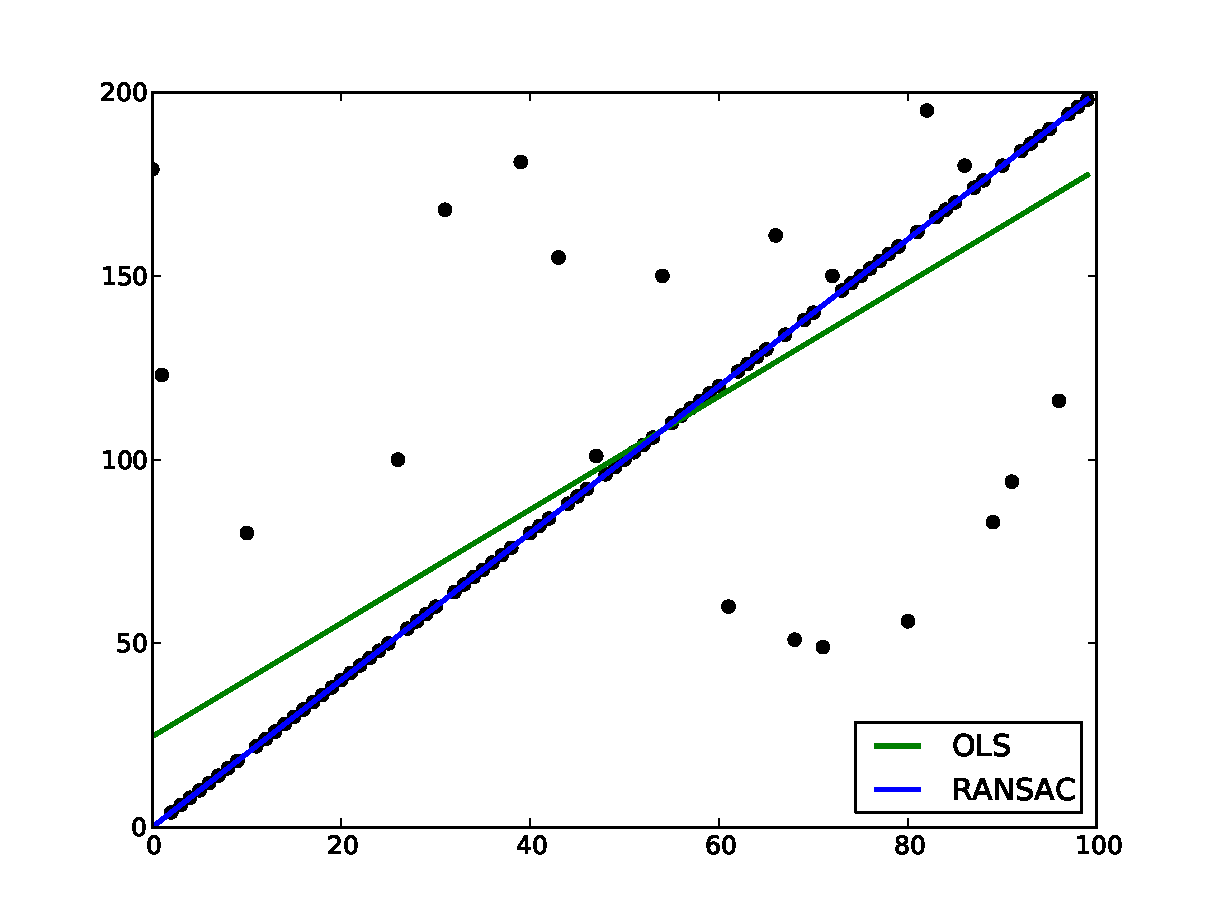
\includegraphics[width=\linewidth]{ransac}
    \caption{The RANSAC algorithm in action.}
\end{figure}

\subsection{Sequence alignment}
Explain the concept of sequence alignment and why it is needed. (We need it
because of fields with variable length)

\subsubsection{Needleman-Wunsch}
Describe the Needleman-Wunsch algorithm for performing global sequence
alignment.

\section{Protocol state inference}

\subsection{Protocol state}
Explain what a protocol state is and how to represent it.

\subsection{State inference}
Explain how we build a state machine from our clusters.

\chapter{Results}

\section{Data sets}
Provide information about the data used to produce the results.

Shouldn't there be a section here?
Display the results of applying our method to different data sets.

\chapter{Discussion}
Discuss why the results are as they are.

\chapter{Conclusions}
Draw conclusions about our method and compare it to the related methods.

\section{Limitations}
Give a short introduction to the different limitations of our method.

\subsection{Textual protocols}
Explain why our method is not applicable to textual protocols.

\subsection{Variable number of fields}
Explain the problem with protocols that contain a variable number of fields and
why our method does not accomodate for them. (Because we based our definition
of protocols on a fixed number of fields?)

\subsection{Non-aligned data}
Explain why we only try to find aligned fields and the problem with complexity
if we were to relax this requirement.

\subsection{Bit precision}
Talk a little bit about how some protocols do not use entire bytes as the sizes
of their fields and that we will not find exact boundaries for them.

\section{Future work}
Mention the ideas that has come up during the thesis work that we have not had
time to investigate further.

\subsection{Correspondence analysis}
Explain how correspondence analysis could give a better result than PCA.

\subsection{Timestamp identification}
Explain how timestamps could potentially be identified from their distinguished
byte distribution pattern.

\bibliographystyle{plain}
\bibliography{thesis}

\end{document}

